\subsection{Relationship Between Cell Size and Growth Rate}
The relationship between cell size and growth rate has long been of interest in
the study of bacterial physiology, particularly following the now six decade-old
observation that cell volume appears to increase exponentially with growth rate;
known as Schaechter's growth law \citep{schaechter1958, taheriaraghi2015}.
However, the mechanism that governs this relationship, and even the question of
whether the change in average cell size is truly exponential, has remained under
debate \citep{harris2018}.  Here we examine the influence of ribosomal content
and total protein abundance on cell size.

Cells grow at a near-maximal rate dictated by their total ribosomal mass
fraction $\Phi_R$, at least at moderate growth rates above 0.5 hr$^{-1}$ (where
$f_a$ is close to 1, and $r_t$ is near its maximal rate).  Here, growth rate can
be increased only by increasing $\Phi_R$, though the simple addition of more
ribosomes is likely constrained by aspects physical constrains like
macromolecular crowding \citep{delarue2018, solerbistue2020}. As \textit{E.
coli} grows faster, large swaths of its proteome increase in absolute abundance.
It is now well-documented that \textit{E. coli} cells add a constant volume per
origin of replication (termed a "unit cell" or "initiation mass"), which is
robust to a remarkable array of cellular perturbations \citep{si2017}. To
consider this dependency in the context of the proteomic data, we used
measurements from \cite{si2017} (\FIG{translation_ecoli_partA}(A)) to estimate the
average number of origins per cell $\langle$\# ori$\rangle$ at different growth rates.
$\langle$\# ori$\rangle$ is set by how often
replication must be initiated per cell doubling under steady-state growth.
This can be quantified as
\begin{equation}
    \langle \text{\# ori} \rangle = 2^{\tau_{cyc} / \tau} = 2^{\tau_{cyc} \lambda / ln(2)},
    \label{eq:Nori}
\end{equation}
where $t_{cyc}$ is the cell cycle time (referring to the time from replication
initiation to cell division), and $\tau$ is the cell doubling time. For
ribosomal synthesis, we find an approximately linear correlation between
ribosome copy number and $\langle$\# ori$\rangle$
(\FIG{translation_ecoli_partA}(B)).

For a constant cell cycle time, observed at growth rates above about 0.5
hr$^{-1}$ \citep{helmstetter1968}, \EQ{Nori} states that $\langle \text{\# ori}
\rangle$ will need to increase exponentially with the growth rate. While this
says nothing of the observed scaling with cell size, the additional dependency
on ribosomal content, which increases with $\langle$\# ori$\rangle$, provides a
link. In \FIG{translation_ecoli_partA}(D), we consider the
position-dependent protein expression across the chromosome by calculating a
running Gaussian average of protein copy number (20 kbp st. dev. averaging
window) based on each gene's transcriptional start site, which were then
median-subtracted to account for the differences in total protein abundance.
Importantly, major deviations in protein copy number are largely restricted to
regions of ribosomal protein genes. This suggests that the relative ribosomal
abundance $\Phi_R$ is also being tuned in proportion to $\langle$\#
ori$\rangle$, with the exponential relationship between  cell size and growth
rate following from how \textit{E. coli} varies its number of ribosomes per
cell.


\begin{figure*}
    \begin{fullwidth}
    \centering{
        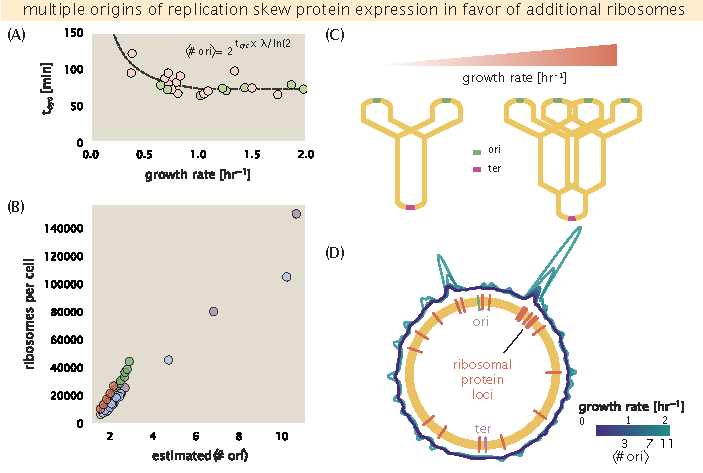
\includegraphics{main_figs/fig8_ribosome_growth_limit_ecoli_a_polar_coord.pdf}
        \caption{\textbf{Cells increase absolute ribosome abundance with
        $\langle$\# ori$\rangle$.} (A) Experimental data from Si \textit{et al.}
        (2017). Dashed line shows fit to the data, which were used to estimate
        $\langle$\# ori$\rangle$. $t_{cyc}$ was assumed to vary in proportion to
        $\tau$ for doubling times greater than 40 minutes, and reach a
        minimum value of 73 minutes (see Appendix
        \nameref{sec:SI_ori} for additional details). Red data points correspond
        to measurements in strain MG1655, while light green points are for
        strain NCM3722. (B) Plot of the ribosome copy number estimated from the
        proteomic data against the estimated $\langle$\# ori$\rangle$. (C)
        Schematic shows the expected increase in replication forks (or number of
        ori regions) as \textit{E. coli} cells grow faster. (D) A running
        Gaussian average (20 kbp st. dev.) of protein copy number is calculated
        for each growth condition considered by \citep{schmidt2016}. Since total
        protein abundance increases with growth rate, protein copy numbers are
        median-subtracted to allow comparison between growth conditions.
        $\langle$\# ori$\rangle$ are estimated using the data in (A) and
        Equation \ref{eq:Nori}. } \label{fig:translation_ecoli_partA}
    }
    \end{fullwidth}
\end{figure*}
